\documentclass{beamer}
\usepackage[utf8]{inputenc}
\usepackage{tcolorbox}
\tcbuselibrary{skins, breakable}

\usetheme{Madrid}
\definecolor{soleneBlue}{RGB}{0, 102, 204}
\definecolor{soleneLightBlue}{RGB}{240, 248, 255}

\title{Interview Presentation}
\author{Solene}
\date{July 17th, 2025}

\begin{document}

\frame{\titlepage}

\begin{frame}
\frametitle{Introduction}
\begin{itemize}
    \item About me
    \item Project Objectives
    \item From Terraform to your GitLab Pipeline through Ansible
    \item Challenges Overcome
    \item Achievements
    \item Agile, Scrum and SysOps
    \item Key practices
    \item Transformation through Automation
\end{itemize}
\end{frame}

\begin{frame}
\frametitle{About me}
\begin{itemize}
    \item \textbf{Started as a Linux System Administrator}  
    \begin{itemize}
        \item \textit{Specializing in building, optimizing, and maintaining Linux-based infrastructures.}
    \end{itemize}

    \item \textbf{Automation Engineer}  
    \begin{itemize}
        \item  \textit{Dedicated to crafting efficient and scalable automated solutions that streamline operations.}
    \end{itemize}

    \item \textbf{DevOps Advocate}  
    \begin{itemize}
       \item  \textit{Bridging the gap between development and operations to foster collaborative and continuous delivery pipelines.}
    \end{itemize}

    \item \textbf{Experienced SysOps on production environments}  
    \begin{itemize}
        \item \textit{Ensuring the reliability, performance, and security of critical systems and services}.  
    \end{itemize}
\end{itemize}
\end{frame}

\begin{frame}
\frametitle{Project Objectives}

\begin{tcolorbox}[colframe=cyan!30, colback=white, arc=3mm, boxrule=0.6pt,
  left=2mm, right=2mm, top=1mm, bottom=1mm, width=\textwidth]
  \textbf{1. Infrastructure provisioning} \\
  \vspace{0.4em}
  Decrease manual processes to have \textbf{idempotent} and \textbf{error-free} deployments across environments.
\end{tcolorbox}

\vspace{0.3em}

\begin{tcolorbox}[colframe=cyan!30, colback=white, arc=3mm, boxrule=0.6pt,
  left=2mm, right=2mm, top=1mm, bottom=1mm, width=\textwidth]
  \textbf{2. IAC* integration} \\
  \vspace{0.4em}
  Connect IAC with CI/CD\footnote{IAC: Infrastructure as Code, CI/CD: Continuous Integration / Continuous Delivery} pipelines for a \textbf{smooth delivery} process.
\end{tcolorbox}

\vspace{0.3em}

\begin{tcolorbox}[colframe=cyan!30, colback=white, arc=3mm, boxrule=0.6pt,
  left=2mm, right=2mm, top=1mm, bottom=1mm, width=\textwidth]
  \textbf{3. Collaboration} \vspace{0.4em} Motivate \textbf{ cross-functional teamwork} to accelerate delivery through automation.
\end{tcolorbox}
\end{frame}

\begin{frame}
\frametitle{From Terraform to your GitLab Pipeline through Ansible}
% Add content here
\end{frame}

\begin{frame}
\frametitle{Challenges Overcome}

\begin{tcolorbox}[colframe=cyan!30, colback=white, arc=3mm, boxrule=0.6pt,
  left=2mm, right=2mm, top=1mm, bottom=1mm, width=\textwidth, enlarge left by=0mm]
  \textbf{Advocate for DevOps principle} \\
  \vspace{0.5em}
  Synchronized complex state across multiple teams and environments
\end{tcolorbox}

\vspace{1em}

\begin{tcolorbox}[colframe=cyan!30, colback=white, arc=3mm, boxrule=0.6pt,
  left=2mm, right=2mm, top=1mm, bottom=1mm, width=\textwidth, enlarge left by=0mm]
  \textbf{Configuration Drift Prevention} \\
  \vspace{0.5em}
  Maintained idempotency while managing intricate infrastructure dependencies
\end{tcolorbox}

\vspace{1em}

\begin{tcolorbox}[colframe=cyan!30, colback=white, arc=3mm, boxrule=0.6pt,
  left=2mm, right=2mm, top=1mm, bottom=1mm, width=\textwidth, enlarge left by=0mm]
  \textbf{Agile Integration} \\
  \vspace{0.5em}
  Aligned automation workflows with sprint cycles and review processes
\end{tcolorbox}
\end{frame}

\begin{frame}
\frametitle{Achievements}

\begin{columns}[T,onlytextwidth]
    
    \column{0.32\textwidth}
    \begin{tcolorbox}[colframe=soleneBlue!30, colback=white, boxrule=0.4pt, arc=1mm, left=1mm, right=1mm, top=0.5mm, bottom=0.5mm]
        \centering
        \textbf{Reduced Manual Work} \\
        \vspace{0.5em}
        \footnotesize Accelerated deployments through comprehensive automation
    \end{tcolorbox}
    
    \column{0.32\textwidth}
    \begin{tcolorbox}[colframe=soleneBlue!30, colback=white, boxrule=0.4pt, arc=1mm, left=1mm, right=1mm, top=0.5mm, bottom=0.5mm]
        \centering
        \textbf{Stability} \\
        \vspace{0.5em}
        \footnotesize Achieved consistent system states with zero configuration drift
    \end{tcolorbox}
    
    \column{0.32\textwidth}
    \begin{tcolorbox}[colframe=soleneBlue!30, colback=white, boxrule=0.4pt, arc=1mm, left=1mm, right=1mm, top=0.5mm, bottom=0.5mm]
        \centering
        \textbf{Speed} \\
        \vspace{0.5em}
        \footnotesize Rapid environment delivery for development and tests
    \end{tcolorbox}

\end{columns}

\end{frame}

\begin{frame}
\frametitle{Agile, Scrum and SysOps}

\centering
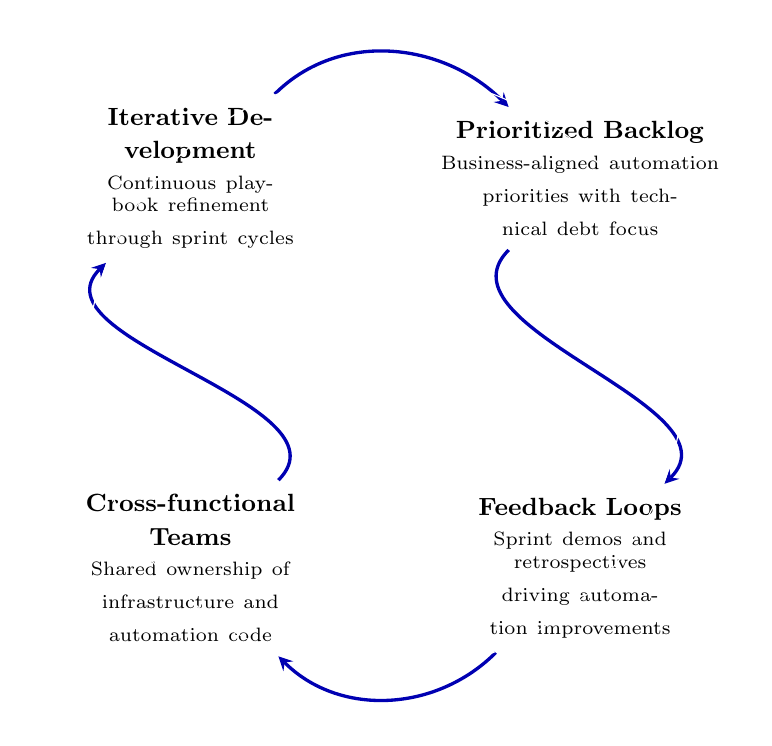
\begin{tikzpicture}[
    item/.style={text width=0.3\textwidth, align=center, inner sep=5pt},
    arrow/.style={->, >=stealth, thick, blue!70!black, line width=1.2pt}
]

\node[item] (A) at (135:3.5cm) {
    \textbf{\small Iterative Development} \\
    \vspace{0.3em}
    \scriptsize Continuous playbook refinement\\ through sprint cycles
};

\node[item] (B) at (45:3.5cm) {
    \textbf{\small Prioritized Backlog} \\
    \vspace{0.3em}
    \scriptsize Business-aligned automation\\ priorities with technical debt focus
};

\node[item] (C) at (-45:3.5cm) { 
    \textbf{\small Feedback Loops} \\
    \vspace{0.3em}
    \scriptsize Sprint demos and retrospectives\\ driving automation improvements
};

\node[item] (D) at (-135:3.5cm) {
    \textbf{\small Cross-functional Teams} \\
    \vspace{0.3em}
    \scriptsize Shared ownership of\\ infrastructure and automation code
};

\draw[arrow] (A) to[out=45,in=135] (B);
\draw[arrow] (B) to[out=-135,in=45] (C);
\draw[arrow] (C) to[out=-135,in=-45] (D);
\draw[arrow] (D) to[out=45,in=-135] (A);

\draw[white] (0,0) circle (3.8cm);
\end{tikzpicture}

\vspace{0.5cm}
\footnotesize
\textit{Combining Agile practices with infrastructure operations}
\end{frame}

\begin{frame}
\frametitle{Key practices}
% Add content here
\end{frame}

\begin{frame}
\frametitle{Transformation through Automation}
% Add content here
\end{frame}

\end{document}
